% 2006 安徽卷理 Q19；正六边形及空间点的仿射投影示意，O 为 BF 中点。
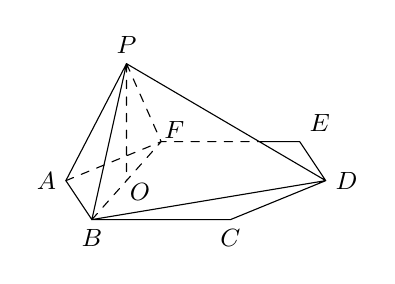
\begin{tikzpicture}[scale=1.1,line cap=round,line join=round,font=\small]
  \coordinate (A) at (0,0);
  \coordinate (B) at (0.3,-0.45);
  \coordinate (C) at (1.9,-0.45);
  \coordinate (D) at (3,0);
  \coordinate (E) at (2.7,0.45);
  \coordinate (F) at (1.1,0.45);
  \coordinate (H) at (2.2333333,0.45); % PD 与 FE 的图示交点，仅用于分段绘线
  \coordinate (O) at (0.7,0);
  \coordinate (P) at (0.7,1.35);

  \draw[dashed] (A)--(F)--(H) (B)--(F) (P)--(F) (P)--(O);
  \draw (H)--(E) (A)--(B)--(C)--(D)--(E) (B)--(D) (P)--(A) (P)--(B) (P)--(D);

  \node[left] at (A) {$A$};
  \node[below] at (B) {$B$};
  \node[below] at (C) {$C$};
  \node[right] at (D) {$D$};
  \node[above right] at (E) {$E$};
  \node[above right,inner sep=1pt] at (F) {$F$};
  \node[below right,inner sep=1pt] at (O) {$O$};
  \node[above] at (P) {$P$};
\end{tikzpicture}
